% State space diagram of the STARTS model (vignette starts).
\documentclass[tikz, border = 6pt]{standalone}
\usepackage{amsmath}
\usepackage{bm}
\usetikzlibrary{arrows.meta, positioning, calc}
\tikzset{
  lat/.style = {circle, draw, thick, minimum size = 13mm, inner sep = 0pt},
  obs/.style = {rectangle, draw, thick, minimum size = 11mm, inner sep = 1pt},
  noise/.style = {circle, draw, minimum size = 9mm, inner sep = 0pt},
  reg/.style = {-{Stealth[length = 2.5mm]}, thick},
  cov/.style = {{Stealth[length = 2mm]}-{Stealth[length = 2mm]}},
  var/.style = {cov, looseness = 5},
  lab/.style = {font = \footnotesize, fill = white, inner sep = 1pt},
  mat/.style = {font = \small, inner sep = 2pt, align = left},
  dots/.style = {font = \Large}
}
\begin{document}
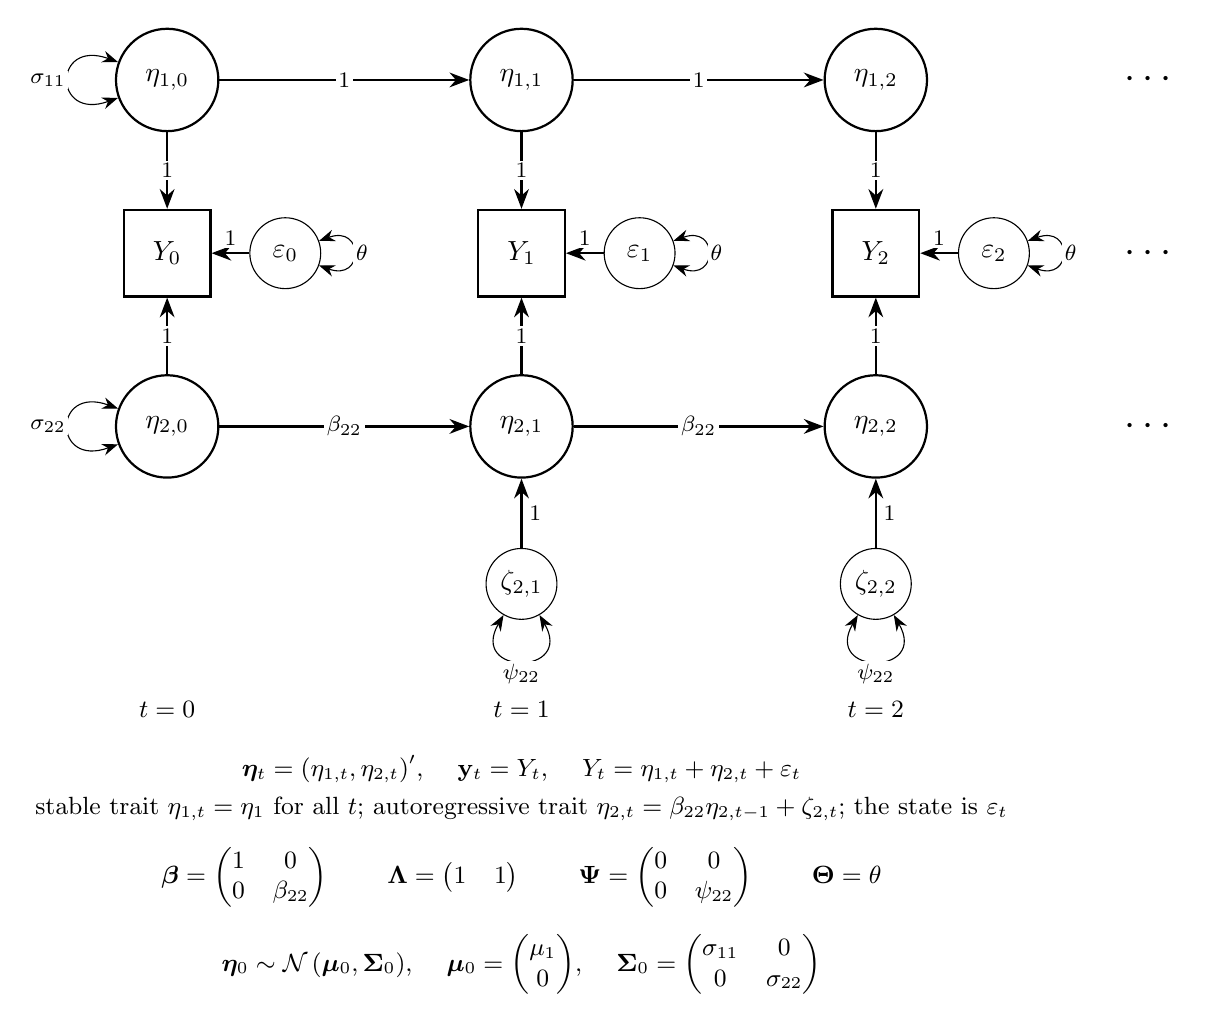
\begin{tikzpicture}
  % occasions
  \foreach \t/\x in {0/0, 1/4.5, 2/9} {
    \node[lat] (a\t) at (\x, 5.0) {$\eta_{1, \t}$};
    \node[obs] (y\t) at (\x, 2.8) {$Y_{\t}$};
    \node[lat] (b\t) at (\x, 0.6) {$\eta_{2, \t}$};
    \node[noise] (u\t) at (\x + 1.5, 2.8) {$\varepsilon_{\t}$};
    \draw[reg] (a\t) -- node[lab] {1} (y\t);
    \draw[reg] (b\t) -- node[lab] {1} (y\t);
    \draw[reg] (u\t) -- node[lab, above = 0.5mm] {1} (y\t);
    \draw[var] (u\t.20) to[out = 20, in = -20]
      node[lab, right] {$\theta$} (u\t.-20);
    \node[font = \small] at (\x, -3.0) {$t = \t$};
  }
  % transitions
  \foreach \s/\t in {0/1, 1/2} {
    \draw[reg] (a\s) -- node[lab, pos = 0.5] {1} (a\t);
    \draw[reg] (b\s) -- node[lab, pos = 0.5] {$\beta_{22}$} (b\t);
  }
  % process noise (autoregressive trait only)
  \foreach \t/\x in {1/4.5, 2/9} {
    \node[noise] (z\t) at (\x, -1.4) {$\zeta_{2, \t}$};
    \draw[reg] (z\t) -- node[lab, right = 0.5mm] {1} (b\t);
    \draw[var] (z\t.240) to[out = 240, in = 300]
      node[lab, below] {$\psi_{22}$} (z\t.300);
  }
  \foreach \r in {5.0, 2.8, 0.6} {
    \node[dots] at (12.5, \r) {$\cdots$};
  }
  % initial condition
  \draw[var] (a0.160) to[out = 160, in = 200]
    node[lab, left] {$\sigma_{11}$} (a0.200);
  \draw[var] (b0.160) to[out = 160, in = 200]
    node[lab, left] {$\sigma_{22}$} (b0.200);
  % matrices
  \node[mat, align = center, below] at (4.5, -3.5) {%
    $\bm{\eta}_{t} = \left( \eta_{1, t}, \eta_{2, t} \right)^{\prime}$,
    \quad $\mathbf{y}_{t} = Y_{t}$, \quad
    $Y_{t} = \eta_{1, t} + \eta_{2, t} + \varepsilon_{t}$ \\[1mm]
    stable trait $\eta_{1, t} = \eta_{1}$ for all $t$;
    autoregressive trait
    $\eta_{2, t} = \beta_{22} \eta_{2, t - 1} + \zeta_{2, t}$;
    the state is $\varepsilon_{t}$ \\[3mm]
    $\bm{\beta} = \begin{pmatrix} 1 & 0 \\ 0 & \beta_{22} \end{pmatrix}$
    \qquad $\bm{\Lambda} = \begin{pmatrix} 1 & 1 \end{pmatrix}$
    \qquad $\bm{\Psi} = \begin{pmatrix} 0 & 0 \\ 0 & \psi_{22}
      \end{pmatrix}$
    \qquad $\bm{\Theta} = \theta$ \\[3mm]
    $\bm{\eta}_{0} \sim \mathcal{N} \left( \bm{\mu}_{0},
      \bm{\Sigma}_{0} \right)$, \quad
    $\bm{\mu}_{0} = \begin{pmatrix} \mu_{1} \\ 0 \end{pmatrix}$, \quad
    $\bm{\Sigma}_{0} = \begin{pmatrix}
      \sigma_{11} & 0 \\ 0 & \sigma_{22}
    \end{pmatrix}$};
\end{tikzpicture}
\end{document}